\documentclass[10pt,a4paper]{report}
\usepackage[utf8]{inputenc}
\usepackage[french]{babel}
\usepackage[T1]{fontenc}
\usepackage{amsmath}
\usepackage{amsfonts}
\usepackage{amssymb}
\usepackage{graphicx}
\usepackage[table,xcdraw]{xcolor}
\usepackage[left=2cm,right=2cm,top=2cm,bottom=2cm]{geometry}
\usepackage{cancel}
\begin{document}
\title{Rapport laboratoire de mesure}
\chapter{}
\section{But}
Le but de cette manipulation est d'analyser l'influence d'une charge placée sur une balance et de mesurer une tension grâce à une pont de Wheatstone avec des capteurs de déformations.La Jauge de déformation a donc pour but de traduire la déformation d'une pièce en variation de résistance électrique. Différentes grandeurs d'influences devront ainsi être analysées comme l'excentration de la charge sur la mesure et de manière théorique, l'influence de la température sur le système. (devellopé dans le chapitre 2 - Montage)

\section{Hypothèse}
\begin{itemize}
\item Influence de la température sur la résistivité et donc sur la mesure.
\item Les matériaux sont homogènes et isotropes - la résistivité reste constante
\item Cylindricité parfaite du corps d'épreuve et rapport ($\mu$) entre le diamètre et la longueur $\rightarrow$ le volume reste constant
\item On supposera le montage réalisé idéal (devellopé dans le chapitre 2 - Montage)
\item On supposera le matériel de mesure fiable
\item On supposera les masses bien étalonnées
\end{itemize}	

\section{Schema fonctionnel}
\begin{center}
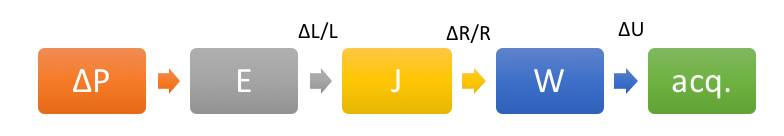
\includegraphics[scale=0.3]{image1.jpg} 
\end{center}

Lorsqu'on applique un effort $\Delta$P au corps d'épreuve, un champ de contraintes apparait dans celui-ci et donc des déformations. Celles-ci sont directement proportionnelles au module de Young de l'aluminium et aux contraintes. Nos jauges résistives, collées sur le corps d'épreuves, subissent les mêmes déformations que le corps. D'après la loi de Pouillet, nous savons que la variation de longueur d'une résistance modifie directement sa valeur. Grâce à un montage de ces jauges en un pont de Weathstone, nous pouvons alors mesurer une différence de tension sur ces résistances et donc obtenir la valeur de la déformation du corps suivant la charge appliquée.


\section{Liste du matériel}
\begin{itemize}
\item 8 jauges de déformations (type FCA-5-23)
\item 1 corps d'épreuve (diabolo en aluminium)
\item 5 charges experimentales de masse connue numérotées ~\\~\\
\begin{tabular}{|c|c|c|c|c|c|}
\hline 
Num & 4 & 5 & 6 & 7 & 9 \\ \hline
Kg    & 0,584 & 1,056 & 1,050 & 1,063 & 1,964 \\ \hline
\end{tabular}~\\
\item un générateur de courant continu (5V)
\item Matériel d'acquisition (Ordinateur avec software dédié)
\item 1 Balance à levier
\item 1 sabot
\end{itemize}
\chapter{Montage}
\section{Type de montage}
\subsection{diviseur de tension}
Dans la pratique, on utilisera le montage en diviseur de tension pour mesurer des différences de potentielles au borne d'une résistance. Cependant dans notre cas, ce montage peut poser des problèmes en terme de précision. Les jauges de déformation présente des variations de 24m$\Omega$ . et donc une variation de tension très faible!
\subsection{Pont de Wheatsone}
Montage qui permet d'avoir une tension nulle à l'équilibre, on mesure donc avec une grande précision les petites variations de tensions. la tension de sortie sera donc proportionnel aux variations relatives $\frac{dr}{R}$ de chacunes des résistances
\subsubsection*{couple de jauges}
\paragraph{}La température influence la résistivité de la jauge. l'origine de cette variation de chaleur pouvant être extérieur ou simplement dûe à effet joule au sein même de la jauge. L'utilisation d'une deuxième jauge placée a proximité et placée dans un montage en pont Wheastone permet de s'affranchir de l'influence de la temperature sur la mesure.
\paragraph{}Par ailleurs, il est recommandé de limiter à 5V la tension d'entrée pour éviter que la chaleur dissipée par la résistance ne diminue la qualité d'adhésion de la colle.
\section{Placement des jauges de déformation}
\subsection{2 jauges perpendiculaires}
Si l'on place les 2 jauges de manière perpendiculaires, on conserve notre mesure de déformation car les deux jauges se deforme différement.
\subsection{4 x 2 jauges perpendiculaires}
\begin{figure}
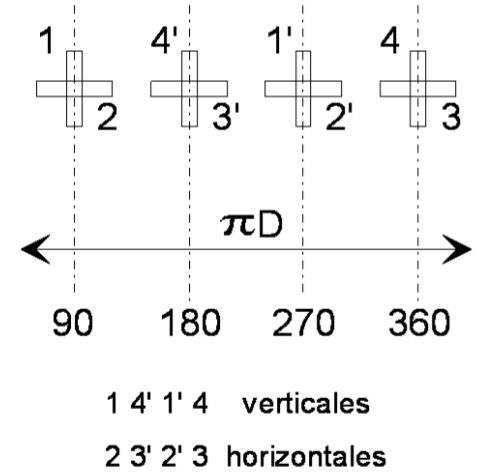
\includegraphics[scale=0.2]{jauge.png} 
\end{figure}
des couples de jauges perpendiculaires seront placées aux quatres points cardinaux du corps d'épreuve afin de reprendre correctement les charges et de ne pas prendre en compte le moment de force qui serait associer à une excentration de la contrainte
\chapter{lien entre tension et déformation}
\section*{Equation  qui lie la tension v à la valeur des résistances des branches du pont de Wheatstone}
\begin{equation}v_{A} = \dfrac{E_{S}(R^{'}_{2}+R_{2})}{(R^{'}_{1}+R_{1})+(R^{'}_{2}+R_{2})}\end{equation} 
\begin{equation}v_{B} = \dfrac{E_{S}(R^{'}_{4}+R_{4})}{(R^{'}_{3}+R_{3})+(R^{'}_{4}+R_{4})} [2]\end{equation} 
\begin{equation}
v = v_{A} - v_{B} = \dfrac{E_{S}((R^{'}_{3}+R_{3})(R^{'}_{2}+R_{2})-(R^{'}_{1}+R_{1})(R^{'}_{4}+R_{4}))}{((R^{'}_{1}+R_{1})+(R^{'}_{2}+R_{2}))((R^{'}_{3}+R_{3})+(R^{'}_{4}+R_{4}))} \end{equation} 

\section*{Calcul de la sollicitation de la jauge}
\begin{equation}
\label{eq:poisson}
\dfrac{dD}{D} = - \mu \dfrac{dL}{L} = - \mu \epsilon =  - \mu \dfrac{\rho}{E}
\end{equation}
\begin{center}où $\mu$ est le facteur de poisson\end{center}
\section*{Loi de Pouillet}
\begin{equation}
\label{eq:pouillet}
R = \rho \dfrac{L}{S}
\end{equation}
\begin{equation}
\label{eq:surface}
 S  = \dfrac{V}{L} 
\end{equation}
\begin{equation}
\label{eq:pouillet2}
\eqref{eq:pouillet}\eqref{eq:surface} \Rightarrow  R = \rho \dfrac{L^{2}}{V}
 \end{equation}
\section*{Calcul du facteur de jauge k}
\begin{equation}
\eqref{eq:pouillet2} \Rightarrow \dfrac{dR}{R} = \dfrac{d(\dfrac{\rho L^{2}}{V})}{\dfrac{\rho L^{2}}{V}} =  \cancel{\dfrac{d\rho}{\rho}}+ \dfrac{2dL}{L}+\cancel{\dfrac{dV}{V}}  =  \dfrac{2dL}{L} \Rightarrow k = 2
\end{equation}
\begin{center}$d\rho$ et $dV$ sont nulles d'après les hypothèses posées précédemment.\end{center}
\section*{donc,}
\begin{equation}
\label{eq:dr}
\eqref{eq:poisson} \eqref{eq:surface} \eqref{eq:pouillet2} \Rightarrow dR = R.k.\frac{\rho}{E} = R.k.\frac{m.g}{E.S}
\end{equation}
\section*{Finalement,}
\begin{equation}
\label{eq:va}
v_{A} = \dfrac{2.E_{S}(R_{0}+\mu dR)}{2.(R_{0}+\mu dR)+2.(R_{0}-\mu dR)}
\end{equation}
\begin{equation}
\label{eq:vb}
v_{B} = \dfrac{2.E_{S}(R_{0}-\mu dR)}{2.(R_{0}+\mu dR)+2.(R_{0}-\mu dR)}
\end{equation}

\begin{equation}
\eqref{eq:va} \eqref{eq:vb} \eqref{eq:dr} \Rightarrow v = v_{A} - v_{B} = \dfrac{E_{S}(\mu dR+dR)}{2.R_{0}+\mu dR -dR} = \dfrac{E_{S}.\cancel{k}.\cancel{R_{0}}\frac{m.g}{E.S}(\mu+1)}{\cancel{2}.\cancel{R_{0}}} = \frac{E_{S}.m.g (\mu + 1)}{E.S}
\end{equation}
\begin{center}
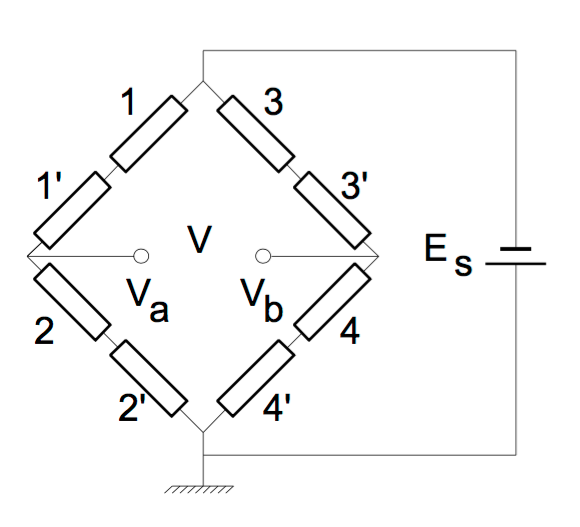
\includegraphics[scale=0.5]{wheatstone.png}
\end{center}
\chapter{Experimentation}

\section{Procédure}
\begin{center}
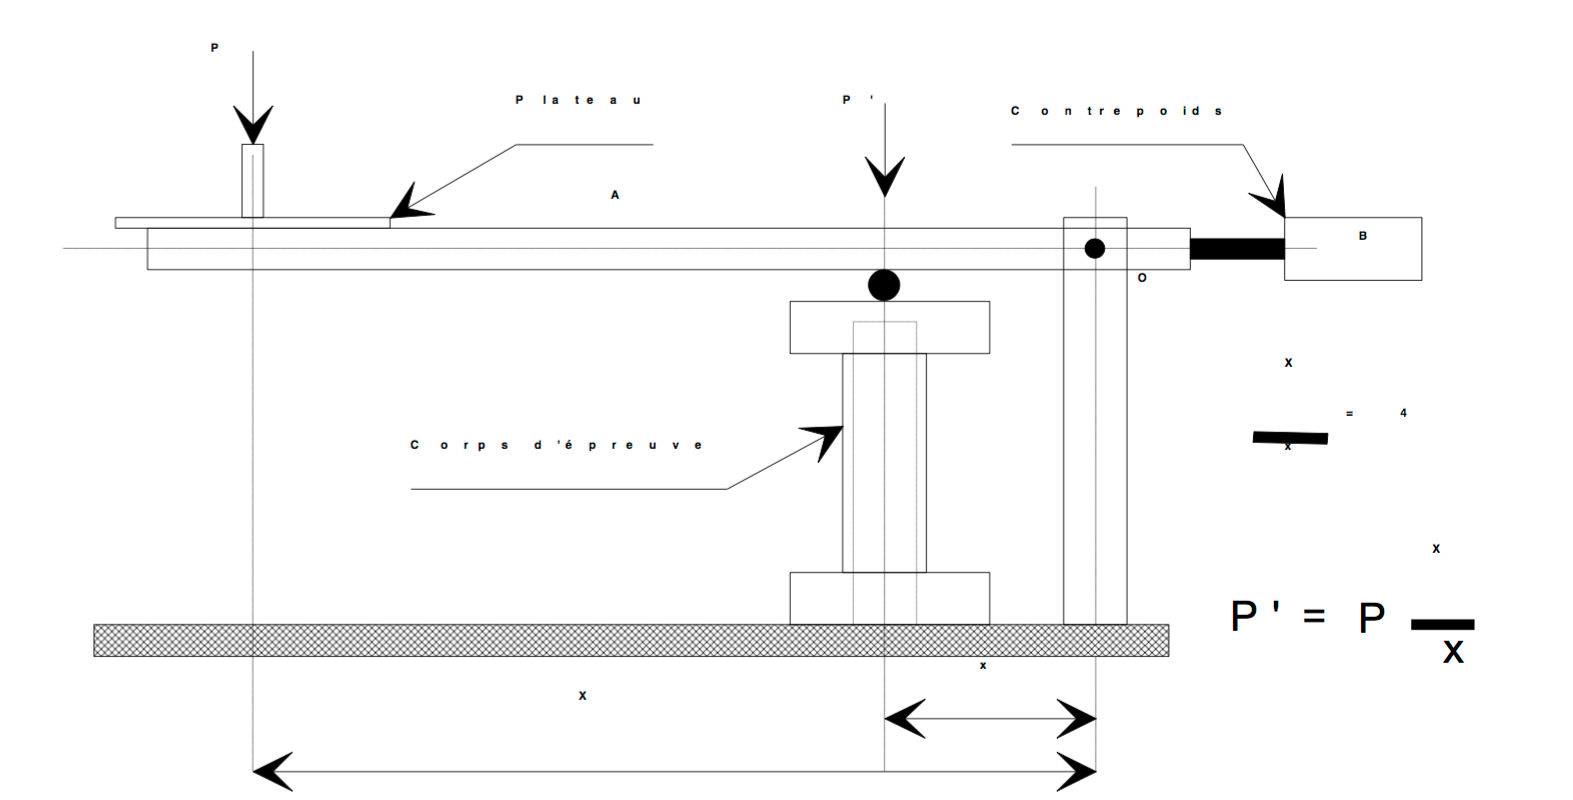
\includegraphics[scale=0.3]{Montage.jpg}
\end{center}
\begin{enumerate}
\item Rééquilibrer le pont de Wheatsone (Calibrage du 0V)
\item Tarrer le masse du système									
\item Centrer le corps d'épreuve sous la bille qui permet d'appliquer la charge.
\item Deposer la charge sur le plateau.
\item Relever la différence de potentiel  et la valeur de la masse affichée à l'écran
\item Répéter les opération 2 à 5 en augmentant la valeur de la charge par pas de 500g en veillant à ne pas déposer une charge supérieur à 5kg
\item Répéter la procédure pour des décentrages de la contrainte (G2/G1/C/D1/D2)
\end{enumerate} 


Il est important de rester délicat avec la matériel lors du changement de masse ou du changement de centrage d'application de la force, Sous peine de fausser les mesures suivantes. S'aider du sabot pour enlever la contrainte sur le diabolo lors du changement de masse.
\newpage
\section{Mesures \& observations}
\subsection*{Graphique}
\begin{center}
~\\
Tension en fonction de la masse lorsque la contrainte est centrée~\\
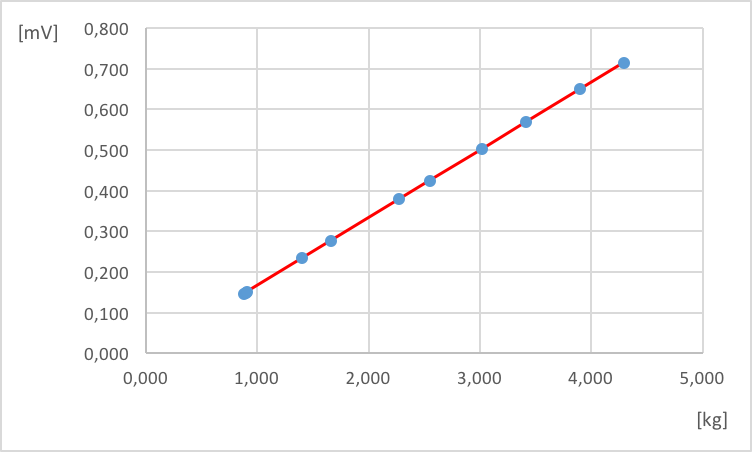
\includegraphics[scale=1]{Graphique1.png} ~\\~\\~\\~\\~\\~\\
Ecart relatif de la masse par rapport à la valeur de la masse lorsque la contrainte est centrée~\\
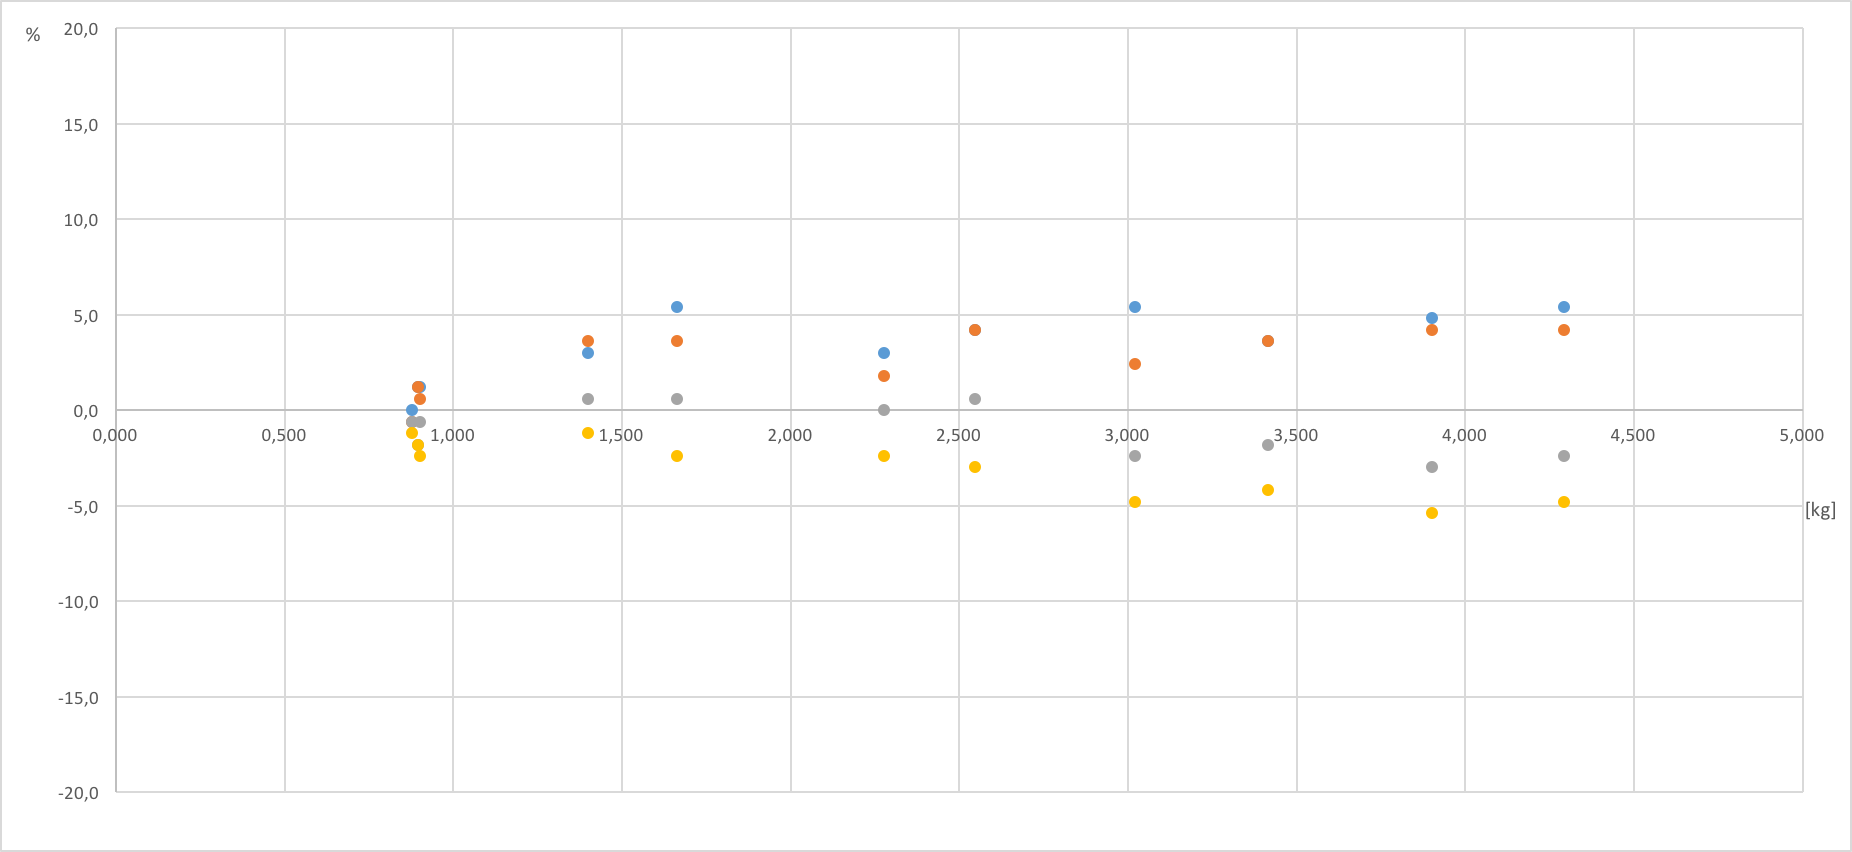
\includegraphics[scale=0.4]{Graphique2.png} ~\\
\end{center}
\newpage
\subsection{Tableau de valeurs}
\begin{center}
~\\
Masse observée en fonction de la masse appliquée et de la position de la contrainte
\begin{tabular}{|c|c|c|c|c|c|c|}
\hline
\rowcolor[HTML]{036400} 
\cellcolor[HTML]{963400}{\color[HTML]{FFFFFF} N}        & \cellcolor[HTML]{963400}{\color[HTML]{FFFFFF} N} & {\color[HTML]{FFFFFF} Masse G2} & {\color[HTML]{FFFFFF} Masse G1} & {\color[HTML]{FFFFFF} Masse C}  & {\color[HTML]{FFFFFF} Masse D1} & {\color[HTML]{FFFFFF} Masse D2} \\ \hline
\rowcolor[HTML]{E7F7E7} 
\cellcolor[HTML]{FFECE2}{\color[HTML]{963400} {[}kg{]}} & \cellcolor[HTML]{FFECE2}{\color[HTML]{963400} }  & {\color[HTML]{036400} {[}kg{]}} & {\color[HTML]{036400} {[}kg{]}} & {\color[HTML]{036400} {[}kg{]}} & {\color[HTML]{036400} {[}kg{]}} & {\color[HTML]{036400} {[}kg{]}} \\ \hline
{\color[HTML]{963400} 0,584}                            & {\color[HTML]{963400} 4}                         & {\color[HTML]{036400} 0,500}    & {\color[HTML]{036400} 0,494}    & {\color[HTML]{036400} 0,512}    & {\color[HTML]{036400} 0,506}    & {\color[HTML]{036400} 0,512}    \\ \hline
{\color[HTML]{963400} 1,050}                            & {\color[HTML]{963400} 6}                         & {\color[HTML]{036400} 0,878}    & {\color[HTML]{036400} 0,884}    & {\color[HTML]{036400} 0,878}    & {\color[HTML]{036400} 0,884}    & {\color[HTML]{036400} 0,890}    \\ \hline
{\color[HTML]{963400} 1,056}                            & {\color[HTML]{963400} 5}                         & {\color[HTML]{036400} 0,884}    & {\color[HTML]{036400} 0,884}    & {\color[HTML]{036400} 0,896}    & {\color[HTML]{036400} 0,914}    & {\color[HTML]{036400} 0,914}    \\ \hline
{\color[HTML]{963400} 1,063}                            & {\color[HTML]{963400} 7}                         & {\color[HTML]{036400} 0,890}    & {\color[HTML]{036400} 0,896}    & {\color[HTML]{036400} 0,902}    & {\color[HTML]{036400} 0,908}    & {\color[HTML]{036400} 0,926}    \\ \hline
{\color[HTML]{963400} 1,640}                            & {\color[HTML]{963400} 4+5}                       & {\color[HTML]{036400} 1,370}    & {\color[HTML]{036400} 1,364}    & {\color[HTML]{036400} 1,400}    & {\color[HTML]{036400} 1,394}    & {\color[HTML]{036400} 1,412}    \\ \hline
{\color[HTML]{963400} 1,964}                            & {\color[HTML]{963400} 9}                         & {\color[HTML]{036400} 1,610}    & {\color[HTML]{036400} 1,628}    & {\color[HTML]{036400} 1,664}    & {\color[HTML]{036400} 1,658}    & {\color[HTML]{036400} 1,688}    \\ \hline
{\color[HTML]{963400} 2,690}                            & {\color[HTML]{963400} 4+5+6}                     & {\color[HTML]{036400} 2,246}    & {\color[HTML]{036400} 2,258}    & {\color[HTML]{036400} 2,276}    & {\color[HTML]{036400} 2,276}    & {\color[HTML]{036400} 2,300}    \\ \hline
{\color[HTML]{963400} 3,020}                            & {\color[HTML]{963400} 5+9}                       & {\color[HTML]{036400} 2,504}    & {\color[HTML]{036400} 2,504}    & {\color[HTML]{036400} 2,546}    & {\color[HTML]{036400} 2,540}    & {\color[HTML]{036400} 2,576}    \\ \hline
{\color[HTML]{963400} 3,604}                            & {\color[HTML]{963400} 5+9+4}                     & {\color[HTML]{036400} 2,966}    & {\color[HTML]{036400} 2,996}    & {\color[HTML]{036400} 3,020}    & {\color[HTML]{036400} 3,044}    & {\color[HTML]{036400} 3,068}    \\ \hline
{\color[HTML]{963400} 4,077}                            & {\color[HTML]{963400} 6+7+9}                     & {\color[HTML]{036400} 3,380}    & {\color[HTML]{036400} 3,380}    & {\color[HTML]{036400} 3,416}    & {\color[HTML]{036400} 3,434}    & {\color[HTML]{036400} 3,458}    \\ \hline
{\color[HTML]{963400} 4,661}                            & {\color[HTML]{963400} 6+7+9+4}                   & {\color[HTML]{036400} 3,854}    & {\color[HTML]{036400} 3,860}    & {\color[HTML]{036400} 3,902}    & {\color[HTML]{036400} 3,932}    & {\color[HTML]{036400} 3,956}    \\ \hline
{\color[HTML]{963400} 5,133}                            & {\color[HTML]{963400} 6+7+9+5}                   & {\color[HTML]{036400} 4,238}    & {\color[HTML]{036400} 4,250}    & {\color[HTML]{036400} 4,292}    & {\color[HTML]{036400} 4,316}    & {\color[HTML]{036400} 4,340}    \\ \hline
\end{tabular}
~\\~\\~\\~\\~\\
Différence de potentielle en fonction de la masse appliquée et de la position de la contrainte~\\
\begin{tabular}{|c|c|c|c|c|c|c|}
\hline
\rowcolor[HTML]{2A2AA1} 
\cellcolor[HTML]{963400}{\color[HTML]{FFFFFF} N}        & \cellcolor[HTML]{963400}{\color[HTML]{FFFFFF} N} & {\color[HTML]{FFFFFF} Tension G2} & {\color[HTML]{FFFFFF} Tension G1} & {\color[HTML]{FFFFFF} Tension C} & {\color[HTML]{FFFFFF} Tension D1} & {\color[HTML]{FFFFFF} Tension D2} \\ \hline
\rowcolor[HTML]{DDDDFF} 
\cellcolor[HTML]{FFECE2}{\color[HTML]{963400} {[}kg{]}} & \cellcolor[HTML]{FFECE2}{\color[HTML]{963400} }  & {\color[HTML]{2A2AA1} {[}mV{]}}   & {\color[HTML]{2A2AA1} {[}mV{]}}   & {\color[HTML]{2A2AA1} {[}mV{]}}  & {\color[HTML]{2A2AA1} {[}mV{]}}   & {\color[HTML]{2A2AA1} {[}mV{]}}   \\ \hline
{\color[HTML]{963400} 0,584}                            & {\color[HTML]{963400} 4}                         & {\color[HTML]{00009B} 0,083}      & {\color[HTML]{00009B} 0,082}      & {\color[HTML]{00009B} 0,085}     & {\color[HTML]{00009B} 0,084}      & {\color[HTML]{00009B} 0,085}      \\ \hline
{\color[HTML]{963400} 1,050}                            & {\color[HTML]{963400} 6}                         & {\color[HTML]{00009B} 0,146}      & {\color[HTML]{00009B} 0,147}      & {\color[HTML]{00009B} 0,146}     & {\color[HTML]{00009B} 0,147}      & {\color[HTML]{00009B} 0,148}      \\ \hline
{\color[HTML]{963400} 1,056}                            & {\color[HTML]{963400} 5}                         & {\color[HTML]{00009B} 0,147}      & {\color[HTML]{00009B} 0,147}      & {\color[HTML]{00009B} 0,149}     & {\color[HTML]{00009B} 0,152}      & {\color[HTML]{00009B} 0,151}      \\ \hline
{\color[HTML]{963400} 1,063}                            & {\color[HTML]{963400} 7}                         & {\color[HTML]{00009B} 0,148}      & {\color[HTML]{00009B} 0,149}      & {\color[HTML]{00009B} 0,150}     & {\color[HTML]{00009B} 0,151}      & {\color[HTML]{00009B} 0,154}      \\ \hline
{\color[HTML]{963400} 1,640}                            & {\color[HTML]{963400} 4+5}                       & {\color[HTML]{00009B} 0,228}      & {\color[HTML]{00009B} 0,227}      & {\color[HTML]{00009B} 0,233}     & {\color[HTML]{00009B} 0,232}      & {\color[HTML]{00009B} 0,235}      \\ \hline
{\color[HTML]{963400} 1,964}                            & {\color[HTML]{963400} 9}                         & {\color[HTML]{00009B} 0,268}      & {\color[HTML]{00009B} 0,271}      & {\color[HTML]{00009B} 0,277}     & {\color[HTML]{00009B} 0,276}      & {\color[HTML]{00009B} 0,281}      \\ \hline
{\color[HTML]{963400} 2,690}                            & {\color[HTML]{963400} 4+5+6}                     & {\color[HTML]{00009B} 0,374}      & {\color[HTML]{00009B} 0,376}      & {\color[HTML]{00009B} 0,379}     & {\color[HTML]{00009B} 0,379}      & {\color[HTML]{00009B} 0,383}      \\ \hline
{\color[HTML]{963400} 3,020}                            & {\color[HTML]{963400} 5+9}                       & {\color[HTML]{00009B} 0,416}      & {\color[HTML]{00009B} 0,417}      & {\color[HTML]{00009B} 0,424}     & {\color[HTML]{00009B} 0,423}      & {\color[HTML]{00009B} 0,429}      \\ \hline
{\color[HTML]{963400} 3,604}                            & {\color[HTML]{963400} 5+9+4}                     & {\color[HTML]{00009B} 0,494}      & {\color[HTML]{00009B} 0,499}      & {\color[HTML]{00009B} 0,502}     & {\color[HTML]{00009B} 0,507}      & {\color[HTML]{00009B} 0,511}      \\ \hline
{\color[HTML]{963400} 4,077}                            & {\color[HTML]{963400} 6+7+9}                     & {\color[HTML]{00009B} 0,563}      & {\color[HTML]{00009B} 0,563}      & {\color[HTML]{00009B} 0,569}     & {\color[HTML]{00009B} 0,572}      & {\color[HTML]{00009B} 0,576}      \\ \hline
{\color[HTML]{963400} 4,661}                            & {\color[HTML]{963400} 6+7+9+4}                   & {\color[HTML]{00009B} 0,642}      & {\color[HTML]{00009B} 0,643}      & {\color[HTML]{00009B} 0,650}     & {\color[HTML]{00009B} 0,654}      & {\color[HTML]{00009B} 0,659}      \\ \hline
{\color[HTML]{963400} 5,133}                            & {\color[HTML]{963400} 6+7+9+5}                   & {\color[HTML]{00009B} 0,706}      & {\color[HTML]{00009B} 0,708}      & {\color[HTML]{00009B} 0,715}     & {\color[HTML]{00009B} 0,718}      & {\color[HTML]{00009B} 0,723}      \\ \hline

\end{tabular}
\end{center}
\paragraph{Observation :} Nous avons constaté qu' au cours de l'expérimentation (après 45min) la valeur du zéro avait légèrement changée (+  0,001 mV pour la mesure de la tension). 
\section{Interpretation}	
\paragraph{} Sur le graphique, on remarque que la progression de la tension en fonction de la contrainte à l'allure d'une droite. Ce qui correspond à l'équation qui lie la tension à la masse  préalablement calculée.(cf formule ...)

\paragraph{}On remarque qu' en fonction de l'excentration de la position de la contrainte il existe une petite variation de la masse affichée sur l'appareil de mesure. Ceci peut-être explique par la poids du levier lui-même qui créé un moment de force différent en fonction de la position du diabolo. 

\paragraph{} Cependant on observe des écart qui reste dans un interevalle de maximum 5\% autour de la valeur lorsque le diabolo est en position centré.

\end{document}
